%%%%%%%%%%%%%%%%%%%%%%%%%%%%%%%%%%%%%%%%%%%%%%%%%%%%%%%%%%%%%%%%%%%%%%%%%%%%%%%
% CSC2059 Practical 6
%%%%%%%%%%%%%%%%%%%%%%%%%%%%%%%%%%%%%%%%%%%%%%%%%%%%%%%%%%%%%%%%%%%%%%%%%%%%%%%

\documentclass{csc2059practical}

% Additional packages used by this practical.
% TikZ is used for the CSC2059 Engineering Workflow diagram.
% FontAwesome is used for the engineering question icon.
\usepackage{tikz}
\usetikzlibrary{arrows.meta, positioning, fit, backgrounds}
\usepackage{fontawesome5}

\setpracticalnumber{6}

\setpracticaltitle{Evolving and Reusing a Generic List}

\setpracticalsubtitle{Understanding Extending Reusing}

\setpracticalauthor{
Dr Giuseppe Trombino\\
School of Electronics, Electrical Engineering and Computer Science\\
Queen's University Belfast
}
\setpracticaldate{}

\usepackage{tikz}
\usetikzlibrary{arrows.meta, positioning, calc, fit}

\definecolor{listnext}{HTML}{2563EB}
\definecolor{listprevious}{HTML}{D97706}
\definecolor{listboundary}{HTML}{15803D}
\definecolor{listnodefill}{HTML}{F3F4F6}


\begin{document}

\maketitle

\tableofcontents
\clearpage

%%%%%%%%%%%%%%%%%%%%%%%%%%%%%%%%%%%%%%%%%%%%%%%%%%%%%%%%%%%%%%%%%%%%%%%%%%%%%%%%
% Introduction
%%%%%%%%%%%%%%%%%%%%%%%%%%%%%%%%%%%%%%%%%%%%%%%%%%%%%%%%%%%%%%%%%%%%%%%%%%%%%%%%

\frontsection{Introduction}

Data structures are rarely built from scratch in professional software development. More often, engineers inherit existing components that have already been tested and integrated into larger systems. Before adding new functionality, it is essential to understand how those components work and to ensure that any changes preserve their existing behaviour.

In this practical, you will work with a generic \mintinline{cpp}{List<T>} implementation that is already used elsewhere in the project. You will begin by exploring how the data structure behaves, then investigate its internal organisation before extending it with new functionality using Test-Driven Development (TDD).

Finally, you will apply your extended implementation to a small railway route planning application. Rather than writing another data structure from scratch, you will reuse the abstraction you have developed to solve a realistic software engineering problem.

\begin{learningoutcomes}
By the end of this practical, you should be able to:

\begin{itemize}
    \item Explain how a doubly linked list maintains bidirectional connections between neighbouring nodes.
    \item Reason about the invariants that keep a linked list in a valid state.
    \item Extend an existing Abstract Data Structure while preserving its public contract.
    \item Use regression tests to verify that new functionality has not broken existing behaviour.
    \item Reuse a generic data structure within a larger software application.
\end{itemize}
\end{learningoutcomes}

\begin{infobox}[Estimated Effort]
This practical should take about 2 hours to complete and is divided in 4 sections.

\begin{itemize}
    \item Part A: estimated completion time = 10 mins;
    \item Part B: estimated completion time = 15 mins;
    \item Part C: estimated completion time = 55 mins; and
    \item Part D: estimated completion time = 40 mins.
\end{itemize}

It also includes some challenges that you should attempt, either if you finish the lab early, or in your own time. 

\end{infobox}


\frontsection{Before You Begin}

Before starting this practical, make sure that you:

\begin{itemize}
    \item have accepted the GitHub Classroom assignment;
    \item have cloned your repository locally;
    \item can build the project successfully using \mintinline{text}{make};
    \item are comfortable running the example programs and public tests from the terminal.
\end{itemize}

\begin{importantnote}
Throughout this practical, follow the CSC2059 Engineering Workflow:

\begin{center}
Predict $\rightarrow$ Observe $\rightarrow$ Understand $\rightarrow$ Test $\rightarrow$ Implement $\rightarrow$ Refine $\rightarrow$ Detect Code Smell $\rightarrow$ Refactor $\rightarrow$ Reuse
\end{center}

Resist the temptation to implement everything at once. Instead, work incrementally, running the supplied demonstrations and public tests frequently as your implementation evolves.
\end{importantnote}


\frontsection{Repository Access}

Open a terminal in the root of your repository and confirm that everything builds correctly:

\begin{terminal}
make
\end{terminal}

This command should compile all example programs and public tests into the \mintinline{text}{bin/} directory.

You can then execute the demonstrations and tests individually throughout the practical using commands such as:

\begin{terminal}
make run-example01
make test01
\end{terminal}


\frontsection{Repository Tour}

Before writing any code, spend a few moments becoming familiar with the repository structure.

\begin{center}
\begin{tabular}{p{0.22\linewidth}p{0.70\linewidth}}
\toprule
\textbf{Folder} & \textbf{Purpose} \\
\midrule
\mintinline{text}{include/} &
Public interfaces for the data structures and application components. \\

\mintinline{text}{src/} &
Implementations of the non-template application components. \\

\mintinline{text}{examples/} &
Small demonstration programs used throughout the practical. \\

\mintinline{text}{tests/} &
Public Catch2 test suites that guide your implementation. \\

\mintinline{text}{data/} &
Datasets used by the demonstration applications. \\

\mintinline{text}{external/} &
Third-party libraries supplied with the repository. \\
\bottomrule
\end{tabular}
\end{center}

\begin{tipbox}
Notice that the repository separates interfaces, implementations, demonstrations and tests into dedicated folders. This organisation is common in larger C++ projects and helps keep related code together as software grows.
\end{tipbox}


\begin{engineeringquestion}[Engineering Journey]

How can an existing data structure be extended with new functionality while preserving the behaviour that other software already depends upon?

Throughout this practical you will investigate how a generic doubly linked list works internally, extend it safely using Test-Driven Development, and finally reuse it within a railway route planning application without modifying the data structure again.
\end{engineeringquestion}


%%%%%%%%%%%%%%%%%%%%%%%%%%%%%%%%%%%%%%%%%%%%%%%%%%%%%%%%%%%%%%%%%%%%%%%%%%%%%%%%
% Part A
%%%%%%%%%%%%%%%%%%%%%%%%%%%%%%%%%%%%%%%%%%%%%%%%%%%%%%%%%%%%%%%%%%%%%%%%%%%%%%%%

\section{Part A: Establishing the Working Baseline}

\begin{learningoutcomes}
By the end of this part, you should be able to:

\begin{itemize}
    \item build and run the supplied \mintinline{cpp}{List<T>} demonstration;
    \item describe the existing behaviour provided by the inherited component;
    \item use regression tests to establish a working baseline before modifying existing software.
\end{itemize}
\end{learningoutcomes}

\begin{infobox}[Estimated Effort]
This section should take about 10 minutes to complete.
\end{infobox}

\subsection{Predict the Existing Behaviour}

The first demonstration creates a \mintinline{cpp}{List<std::string>} with the following railway stations:

\begin{center}
Belfast, Lisburn, Portadown, and Newry
\end{center}

The program then traverses the same \mintinline{cpp}{List<std::string>} twice:

\begin{itemize}
    \item first from Belfast towards Newry;
    \item then from Newry back towards Belfast.
\end{itemize}

Before running the program, predict the order in which the stations should be displayed during each journey.

\begin{reflectionbox}
Write down the expected outward and return orders before continuing.

What capability must the underlying data structure provide to allow the same collection of stations to be traversed efficiently in both directions?
\end{reflectionbox}


\subsection{Observe the Existing List}

Now run the first demonstration:

\begin{terminal}
make run-example01
\end{terminal}

Compare the output with your prediction.

Did the stations appear in the order you expected in both directions?


\subsection{Inspect the Demonstration}

Open:

\begin{terminal}
examples/example01_bidirectional_traversal.cpp
\end{terminal}

Notice that the application creates a generic list containing strings:

\begin{cppcode}
List<std::string> stops;
\end{cppcode}

The route is traversed forwards using:

\begin{cppcode}
stops.setp_first();
stops.get_next();
\end{cppcode}

The same route is then traversed backwards using:

\begin{cppcode}
stops.setp_last();
stops.get_prev();
\end{cppcode}

At this stage, you do not need to understand how these operations are implemented. The important observation is that the inherited component already provides useful, working behaviour.


\subsection{Verify the Existing Contract}

Before extending existing software, engineers first establish that its current behaviour is correct.

Run the existing behaviour tests:

\begin{terminal}
make test01
\end{terminal}

You should see all tests and assertions pass.

\begin{infobox}
\textbf{Regression Tests}

Regression tests protect behaviour that already works. After a component is changed, these tests are run again to detect whether the new implementation has accidentally broken functionality that existing software may depend upon.

The tests in \mintinline{text}{test01_existing_behaviour.cpp} therefore establish the current public contract of \mintinline{cpp}{List<T>}.
\end{infobox}

Open the test file:

\begin{terminal}
tests/test01_existing_behaviour.cpp
\end{terminal}

The tests confirm that the existing implementation supports:

\begin{itemize}
    \item creating an empty list;
    \item inserting items at the front, end and a selected position;
    \item removing items from different positions;
    \item storing more than one type of data;
    \item traversing forwards and backwards.
\end{itemize}

These tests are already green. Your responsibility throughout the remainder of the practical is to keep them green.


\begin{importantnote}
Do not modify \mintinline{text}{test01_existing_behaviour.cpp}.

These tests describe behaviour that other software may already rely upon. After every significant change to \mintinline{cpp}{List<T>}, run:

\begin{terminal}
make test01
\end{terminal}

New functionality is only successful if the existing behaviour continues to pass.
\end{importantnote}


\begin{reflectionbox}
The \mintinline{cpp}{List<T>} implementation is already working.

Why is it safer to establish this baseline before examining or modifying its internal implementation?

Consider what a failing regression test would tell you after a future change.
\end{reflectionbox}


\subsection{Engineering Takeaway}

Working software has an existing contract.

\begin{importantnote}
Before extending a component, establish what already works and protect that behaviour with regression tests. New functionality should increase what the component can do without damaging what it could do before.
\end{importantnote}

% =============================================================================
% Part B
% =============================================================================

\section{Part B: Looking Under the Bonnet}

\begin{learningoutcomes}
By the end of this part, you should be able to:

\begin{itemize}
    \item describe how neighbouring nodes in a doubly linked list are connected;
    \item explain the purpose of the first and last pointers;
    \item explain how the same structure supports forward and backward traversal;
    \item identify the structural rules that must remain true for a valid
          \mintinline{cpp}{List<T>}.
\end{itemize}
\end{learningoutcomes}

\begin{infobox}[Estimated Effort]
This section should take about 15 minutes to complete.
\end{infobox}


\subsection{From Behaviour to Structure}

In Part A, you treated \mintinline{cpp}{List<T>} as a black box. You observed what the component could do without examining how it achieved that behaviour.

Before extending the implementation, you now need to look under the bonnet.

The second demonstration constructs the List one node at a time. It pauses after each important change so that you can compare the program output with the corresponding diagram in this guide.

\begin{importantnote}
Work through the demonstration and this guide together.

Each time the program pauses:

\begin{enumerate}
    \item return to the next checkpoint in this guide;
    \item study the diagram;
    \item answer the accompanying question;
    \item continue the demonstration.
\end{enumerate}

Do not run the entire demonstration first. The purpose of the pauses is to let you update your mental model one step at a time.
\end{importantnote}

\subsection{Begin the Guided Demonstration}

Run:

\begin{terminal}
make run-example02
\end{terminal}

The program will introduce the demonstration and then pause before creating the first node.

Leave the program waiting and continue with Checkpoint 1 below.

\subsection{Checkpoint 1: The Empty List}

Before any nodes are created, the List contains no data.

Its two boundary pointers therefore identify no nodes:

\begin{figure}[htbp]
    \centering
    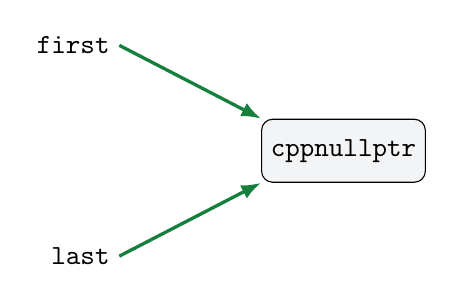
\begin{tikzpicture}[
        boundary/.style={-{Latex[length=2.5mm]}, very thick, listboundary},
        nullvalue/.style={
            draw,
            rounded corners,
            minimum width=2.0cm,
            minimum height=0.8cm,
            fill=listnodefill,
            font=\ttfamily
        }
    ]
        \node[nullvalue] (null) {\mintinline{cpp}{nullptr}};
        \node[above left=0.7cm and 1.8cm of null, font=\ttfamily] (first) {first};
        \node[below left=0.7cm and 1.8cm of null, font=\ttfamily] (last) {last};

        \draw[boundary] (first.east) -- (null.north west);
        \draw[boundary] (last.east) -- (null.south west);
    \end{tikzpicture}

    \caption{The List before any nodes have been created.}
    \label{fig:list-empty}
\end{figure}

For an empty List:

\begin{cppcode}
first == nullptr
last  == nullptr
size  == 0
\end{cppcode}

There is no first node and no last node because there are no nodes at all.

\begin{reflectionbox}
How can the implementation determine whether the List is empty?

Why must both boundary pointers agree about this state?
\end{reflectionbox}

Return to the terminal and continue the demonstration until it pauses again.

\subsection{Checkpoint 2: Creating the First Node}

The program has now inserted \mintinline{text}{Belfast}.

A List containing one node has a special structure:

\begin{figure}[htbp]
    \centering
    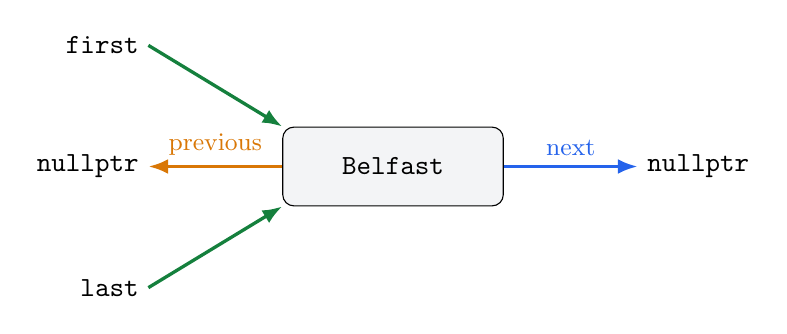
\begin{tikzpicture}[
        node distance=1.5cm,
        listnode/.style={
            draw,
            rounded corners,
            minimum width=2.8cm,
            minimum height=1.0cm,
            fill=listnodefill,
            font=\ttfamily
        },
        boundary/.style={-{Latex[length=2.5mm]}, very thick, listboundary},
        nextlink/.style={-{Latex[length=2.5mm]}, very thick, listnext},
        previouslink/.style={-{Latex[length=2.5mm]}, very thick, listprevious},
        nullvalue/.style={font=\ttfamily}
    ]
        \node[listnode] (belfast) {Belfast};
        \node[above left=0.8cm and 1.7cm of belfast, font=\ttfamily] (first) {first};
        \node[below left=0.8cm and 1.7cm of belfast, font=\ttfamily] (last) {last};
        \node[left=1.7cm of belfast, nullvalue] (leftnull) {nullptr};
        \node[right=1.7cm of belfast, nullvalue] (rightnull) {nullptr};

        \draw[boundary] (first.east) -- (belfast.north west);
        \draw[boundary] (last.east) -- (belfast.south west);
        \draw[previouslink] (belfast.west) --
            node[above, font=\small] {previous}
            (leftnull.east);
        \draw[nextlink] (belfast.east) --
            node[above, font=\small] {next}
            (rightnull.west);
    \end{tikzpicture}

    \caption{A List containing one node.}
    \label{fig:list-first-node}
\end{figure}

Both boundary pointers identify the same node:

\begin{cppcode}
first == last
\end{cppcode}

The first node has no previous neighbour, and the last node has no next neighbour. Since this node is both first and last, both links lead to \mintinline{cpp}{nullptr}.

\begin{reflectionbox}
Why must \mintinline{text}{first} and \mintinline{text}{last} both identify Belfast?

What would be inconsistent about a one-node List in which only one of these boundary pointers was updated?
\end{reflectionbox}

Return to the terminal and continue the demonstration until it pauses again.

\subsection{Checkpoint 3: Connecting a Second Node}

The program has now appended \mintinline{text}{Lisburn}.

The List must establish two relationships between the neighbouring nodes:

\begin{figure}[htbp]
    \centering
    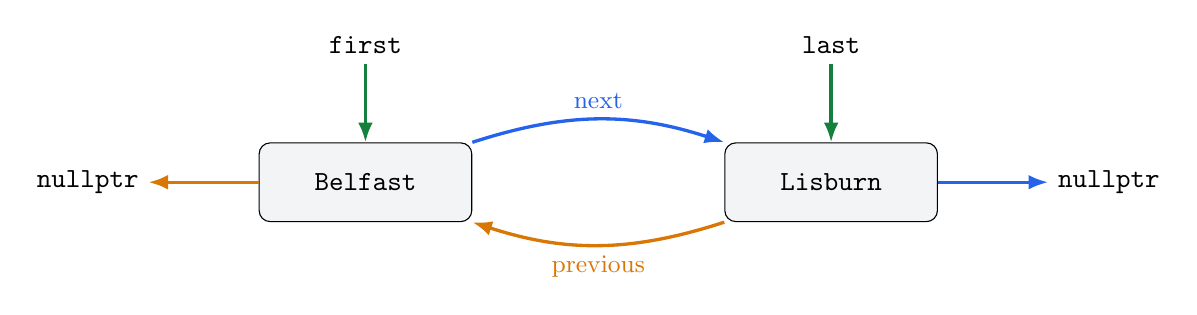
\begin{tikzpicture}[
        node distance=3.2cm,
        listnode/.style={
            draw,
            rounded corners,
            minimum width=2.7cm,
            minimum height=1.0cm,
            fill=listnodefill,
            font=\ttfamily
        },
        boundary/.style={-{Latex[length=2.5mm]}, very thick, listboundary},
        nextlink/.style={-{Latex[length=2.5mm]}, very thick, listnext},
        previouslink/.style={-{Latex[length=2.5mm]}, very thick, listprevious}
    ]
        \node[listnode] (belfast) {Belfast};
        \node[listnode, right=of belfast] (lisburn) {Lisburn};
        \node[above=1.0cm of belfast, font=\ttfamily] (first) {first};
        \node[above=1.0cm of lisburn, font=\ttfamily] (last) {last};
        \node[left=1.4cm of belfast, font=\ttfamily] (leftnull) {nullptr};
        \node[right=1.4cm of lisburn, font=\ttfamily] (rightnull) {nullptr};

        \draw[boundary] (first.south) -- (belfast.north);
        \draw[boundary] (last.south) -- (lisburn.north);
        \draw[previouslink] (belfast.west) -- (leftnull.east);
        \draw[nextlink]
            (belfast.north east)
            to[bend left=18]
            node[above, font=\small] {next}
            (lisburn.north west);
        \draw[previouslink]
            (lisburn.south west)
            to[bend left=18]
            node[below, font=\small] {previous}
            (belfast.south east);
        \draw[nextlink] (lisburn.east) -- (rightnull.west);
    \end{tikzpicture}

    \caption{Two neighbouring nodes connected in both directions.}
    \label{fig:list-two-nodes}
\end{figure}

The blue relationship allows traversal towards the end of the List:

\begin{cppcode}
Belfast.next == Lisburn
\end{cppcode}

The orange relationship allows traversal towards the beginning:

\begin{cppcode}
Lisburn.previous == Belfast
\end{cppcode}

These are not two independent facts. Together, they describe one consistent relationship between neighbouring nodes.

\begin{reflectionbox}
Suppose \mintinline{text}{Belfast.next} identifies Lisburn, but
\mintinline{text}{Lisburn.previous} does not identify Belfast.

Would forward traversal still appear to work?

What might happen during backward traversal?
\end{reflectionbox}

Return to the terminal and continue the demonstration until it pauses again.

\subsection{Checkpoint 4: Building the Two-Way Chain}

The program has now appended \mintinline{text}{Portadown}.

The complete three-node structure is shown below.

\begin{figure}[htbp]
    \centering
    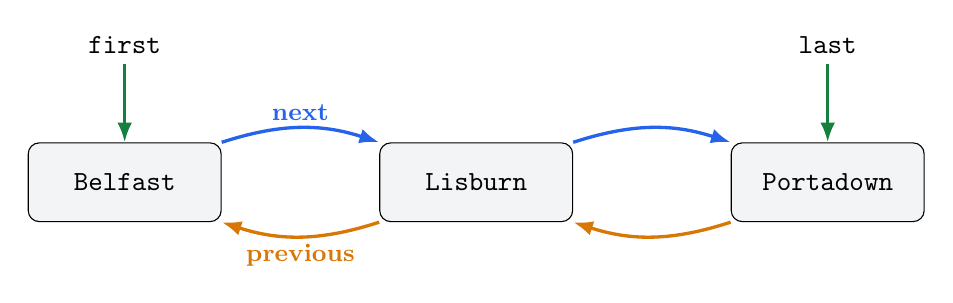
\begin{tikzpicture}[
        node distance=2.0cm,
        listnode/.style={
            draw,
            rounded corners,
            minimum width=2.45cm,
            minimum height=1.0cm,
            fill=listnodefill,
            font=\ttfamily
        },
        boundary/.style={-{Latex[length=2.5mm]}, very thick, listboundary},
        nextlink/.style={-{Latex[length=2.5mm]}, very thick, listnext},
        previouslink/.style={-{Latex[length=2.5mm]}, very thick, listprevious}
    ]
        \node[listnode] (belfast) {Belfast};
        \node[listnode, right=of belfast] (lisburn) {Lisburn};
        \node[listnode, right=of lisburn] (portadown) {Portadown};
        \node[above=1.0cm of belfast, font=\ttfamily] (first) {first};
        \node[above=1.0cm of portadown, font=\ttfamily] (last) {last};


        \draw[boundary] (first.south) -- (belfast.north);
        \draw[boundary] (last.south) -- (portadown.north);
        \draw[nextlink]
            (belfast.north east)
            to[bend left=18]
            (lisburn.north west);
        \draw[previouslink]
            (lisburn.south west)
            to[bend left=18]
            (belfast.south east);
        \draw[nextlink]
            (lisburn.north east)
            to[bend left=18]
            (portadown.north west);
        \draw[previouslink]
            (portadown.south west)
            to[bend left=18]
            (lisburn.south east);

        \node[
            above=0.15cm of $(belfast.north east)!0.5!(lisburn.north west)$,
            text=listnext,
            font=\small\bfseries
        ] {next};

        \node[
            below=0.15cm of $(belfast.south east)!0.5!(lisburn.south west)$,
            text=listprevious,
            font=\small\bfseries
        ] {previous};
    \end{tikzpicture}

    \caption{The same List represented as two consistent chains.}
    \label{fig:list-three-nodes}
\end{figure}

The blue links form a chain from the first node to the last node.

The orange links form a chain from the last node back to the first.

The middle node participates in both chains:

\begin{cppcode}
Lisburn.previous == Belfast
Lisburn.next     == Portadown
\end{cppcode}

\begin{infobox}
The diagram uses a consistent visual language throughout this practical:

\begin{itemize}
    \item \textcolor{listboundary}{\textbf{green}} identifies the external
          \mintinline{text}{first} and \mintinline{text}{last} pointers;
    \item \textcolor{listnext}{\textbf{blue}} identifies
          \mintinline{text}{next} links;
    \item \textcolor{listprevious}{\textbf{orange}} identifies
          \mintinline{text}{previous} links.
\end{itemize}

When the List is modified later, both the blue and orange relationships must remain correct.
\end{infobox}

\begin{reflectionbox}
How many relationships had to be updated when Portadown was appended?

Why is updating only the blue relationship insufficient?
\end{reflectionbox}

Return to the terminal and allow the demonstration to complete.

\subsection{Checkpoint 5: Traversing the Same Structure}

The final scene traverses the List in both directions.

The structure itself does not change. Only the starting point and the links being followed change.

\begin{figure}[htbp]
    \centering
    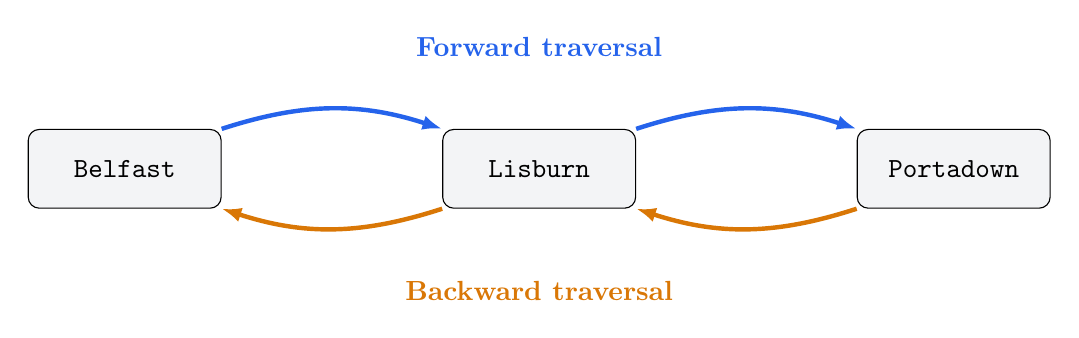
\begin{tikzpicture}[
        node distance=2.8cm,
        listnode/.style={
            draw,
            rounded corners,
            minimum width=2.45cm,
            minimum height=1.0cm,
            fill=listnodefill,
            font=\ttfamily
        },
        nextlink/.style={-{Latex[length=2.5mm]}, ultra thick, listnext},
        previouslink/.style={-{Latex[length=2.5mm]}, ultra thick, listprevious}
    ]
        \node[listnode] (belfast) {Belfast};
        \node[listnode, right=of belfast] (lisburn) {Lisburn};
        \node[listnode, right=of lisburn] (portadown) {Portadown};

        \draw[nextlink]
            (belfast.north east)
            to[bend left=18]
            (lisburn.north west);
        \draw[nextlink]
            (lisburn.north east)
            to[bend left=18]
            (portadown.north west);
        \draw[previouslink]
            (portadown.south west)
            to[bend left=18]
            (lisburn.south east);
        \draw[previouslink]
            (lisburn.south west)
            to[bend left=18]
            (belfast.south east);

        \node[above=0.8cm of lisburn, text=listnext, font=\bfseries]
            {Forward traversal};
        \node[below=0.8cm of lisburn, text=listprevious, font=\bfseries]
            {Backward traversal};
    \end{tikzpicture}

    \caption{Two traversal algorithms using the same underlying structure.}
    \label{fig:list-traversal}
\end{figure}

Forward traversal begins at the first node and repeatedly follows the blue links:

\begin{cppcode}
stops.setp_first();
stops.get_next();
\end{cppcode}

Backward traversal begins at the last node and repeatedly follows the orange links:

\begin{cppcode}
stops.setp_last();
stops.get_prev();
\end{cppcode}

No nodes are rearranged between the two traversals.

\begin{engineeringquestion}
What makes backward traversal practical in this implementation?

How would the operation differ if each node stored only a next link?
\end{engineeringquestion}

\subsection{The Structural Invariants}

The relationships you have observed are not optional implementation details. They are rules that must remain true whenever the List is in a valid state.

Such rules are called \textbf{invariants}.

For every neighbouring pair of nodes \(A\) and \(B\):

\begin{cppcode}
A.next == B
B.previous == A
\end{cppcode}

At the List boundaries:

\begin{cppcode}
first.previous == nullptr
last.next      == nullptr
\end{cppcode}

For an empty List:

\begin{cppcode}
first == nullptr
last  == nullptr
size  == 0
\end{cppcode}

For a one-node List:

\begin{cppcode}
first == last
\end{cppcode}

\begin{importantnote}
A linked operation is not correct merely because the expected values can be printed in one direction.

A valid operation must preserve:

\begin{itemize}
    \item the forward chain;
    \item the backward chain;
    \item the first and last boundaries;
    \item the recorded List size.
\end{itemize}
\end{importantnote}

\begin{commonerror}
\textbf{Updating only one direction}

A common linked-list error is to reconnect the blue \mintinline{text}{next} link but forget the corresponding orange \mintinline{text}{previous} link.

Forward traversal may still appear correct, hiding the damage. Backward traversal exposes the broken relationship.

This is why the public tests in Part C verify the List in both directions.
\end{commonerror}

\begin{reflectionbox}
Imagine removing one or more nodes from the middle of the List.

Which blue relationship would need to change?

Which orange relationship would need to change?

What additional changes might be required if the removed range included the first or last node?
\end{reflectionbox}

\subsection{Engineering Takeaway}

\begin{importantnote}
Engineers do not modify links independently.

Every structural operation must preserve the relationships that allow the whole data structure to function. In a doubly linked list, this means maintaining two consistent chains: one forwards and one backwards.
\end{importantnote}

% =============================================================================
% Part C
% =============================================================================

\section{Part C: Extending the List Safely}

\begin{learningoutcomes}
By the end of this part, you should be able to:

\begin{itemize}
    \item interpret public tests as executable specifications;
    \item transfer a contiguous chain of nodes between two Lists;
    \item preserve forward and backward List invariants during structural changes;
    \item reject invalid requests without modifying either List;
    \item use regression tests continuously while extending an existing component.
\end{itemize}
\end{learningoutcomes}

\begin{infobox}[Estimated Effort]
This section should take about 55 minutes to complete.
\end{infobox}


\subsection{From Understanding to Responsibility}

In Part B, you examined how the inherited \mintinline{cpp}{List<T>} maintains two consistent chains of links.

You will now extend that component with two new operations:

\begin{cppcode}
bool extract(
    int firstPosition,
    int lastPosition,
    List<T>& destination);

bool insert(
    int position,
    List<T>& source);
\end{cppcode}

These operations transfer existing nodes between Lists. They do not copy each stored value into newly created nodes.

This means that your implementation must preserve the structural invariants of every List involved.


\subsection{Observe the Starting Point}

The required behaviour has already been described in:

\begin{terminal}
tests/test02_new_features.cpp
\end{terminal}

Before changing the implementation, run the new functionality tests:

\begin{terminal}
make test02
\end{terminal}

At the start of this part, you should see:

\begin{terminal}
14 test cases
6 passed
8 failed
\end{terminal}

The six passing cases do not mean that part of the new functionality has already been implemented.

Both starter functions currently return \mintinline{cpp}{false} without modifying either List. This means that tests expecting an invalid request to be rejected already pass.

The eight failing tests describe the successful extraction and insertion behaviour that you must now implement.

\begin{engineeringquestion}
The starter implementation rejects every request and therefore cannot corrupt either List.

How can you gradually introduce successful behaviour without losing that safety?
\end{engineeringquestion}


\subsection{Protect the Existing Contract}

Before beginning Part C, confirm that the inherited behaviour remains green:

\begin{terminal}
make test01
\end{terminal}

Throughout this part, you are working with two different test suites:

\begin{center}
\begin{tabular}{p{0.32\linewidth}p{0.58\linewidth}}
\toprule
\textbf{Test Suite} & \textbf{Purpose} \\
\midrule
\mintinline{text}{test01_existing_behaviour.cpp} &
Protects the public contract that already existed before this practical. \\

\mintinline{text}{test02_new_features.cpp} &
Describes the new extraction and insertion behaviour that you are adding. \\
\bottomrule
\end{tabular}
\end{center}

\begin{importantnote}
New functionality is only successful when both test suites pass.

After every meaningful implementation step, run:

\begin{terminal}
make test01
\end{terminal}

A passing new test does not compensate for breaking existing behaviour.
\end{importantnote}


\subsection{Work in Small Steps}

Do not attempt to implement both functions completely before running the tests.

Instead, follow this cycle:

\begin{center}
Run one test group
$\rightarrow$
Inspect the failure
$\rightarrow$
Make one small change
$\rightarrow$
Compile (make)
$\rightarrow$
Run the same test group
$\rightarrow$
Run the regression tests
\end{center}

\begin{importantnote}
Resist the temptation to write the entire implementation first and test it afterwards.

When several links, boundary pointers and size values are changed at once, a failure becomes much harder to diagnose. Small changes keep each failure connected to the code you have just written.
\end{importantnote}

Begin with only the simplest extraction test:

\begin{terminal}
make
./bin/test02_new_features "[extract][core]"
\end{terminal}

Once that case passes, move to:

\begin{terminal}
make
./bin/test02_new_features "[extract][boundary]"
\end{terminal}

Only after the valid extraction cases pass should you run:

\begin{terminal}
make
./bin/test02_new_features "[extract][defensive]"
\end{terminal}

\begin{tipbox}
Remember that the test executable is compiled from your source code.

After every change to \mintinline{cpp}{List.h}, rebuild the project before rerunning the tests:

\begin{terminal}
make
./bin/test02_new_features "[extract][core]"
\end{terminal}

\textbf{If you forget to rebuild, you will simply be rerunning the previous executable rather than testing your latest implementation.}
\end{tipbox}


% -----------------------------------------------------------------------------
% extract()
% -----------------------------------------------------------------------------

\subsection{Extracting a Range of Nodes}

Open:

\begin{terminal}
include/List.h
\end{terminal}

Locate the starter implementation of:

\begin{cppcode}
bool extract(
    int firstPosition,
    int lastPosition,
    List<T>& destination);
\end{cppcode}

The positions describe an inclusive range.

For example:

\begin{cppcode}
source.extract(2, 3, destination);
\end{cppcode}

extracts the nodes at positions \mintinline{cpp}{2} and \mintinline{cpp}{3}.


\subsection{Understand the Contract}

On success, \mintinline{cpp}{extract()} must:

\begin{itemize}
    \item detach the requested range from the source List;
    \item transfer those same nodes into \mintinline{text}{destination};
    \item reconnect the nodes that remain in the source List;
    \item establish valid first and last boundaries in both Lists;
    \item update both List sizes;
    \item return \mintinline{cpp}{true}.
\end{itemize}

No stored values should be copied.

On failure:

\begin{itemize}
    \item the source List must remain unchanged;
    \item the destination List must remain unchanged;
    \item the function must return \mintinline{cpp}{false}.
\end{itemize}

The operation must reject a request when:

\begin{itemize}
    \item either position is outside the source List;
    \item \mintinline{text}{firstPosition} is greater than
          \mintinline{text}{lastPosition};
    \item the destination List is not empty;
    \item the destination is the same object as the source.
\end{itemize}

\begin{tipbox}
Validate the complete request before changing any links.

If you begin modifying the source List and only later discover that the destination is invalid, restoring the original structure becomes considerably more difficult.
\end{tipbox}


\subsection{Visualise an Interior Extraction}

Consider the following source List:

\begin{center}
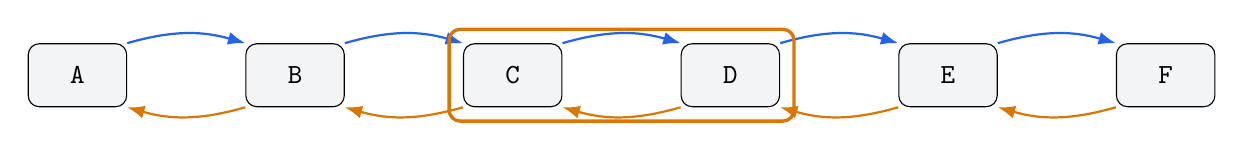
\begin{tikzpicture}[
    node distance=1.5cm,
    listnode/.style={
        draw,
        rounded corners,
        minimum width=1.25cm,
        minimum height=0.8cm,
        fill=listnodefill,
        font=\ttfamily
    },
    nextlink/.style={
        -{Latex[length=2.2mm]},
        thick,
        listnext
    },
    previouslink/.style={
        -{Latex[length=2.2mm]},
        thick,
        listprevious
    },
    selected/.style={
        draw=listprevious,
        very thick,
        rounded corners,
        inner sep=5pt
    }
]
    \node[listnode] (a) {A};
    \node[listnode, right=of a] (b) {B};
    \node[listnode, right=of b] (c) {C};
    \node[listnode, right=of c] (d) {D};
    \node[listnode, right=of d] (e) {E};
    \node[listnode, right=of e] (f) {F};

    \draw[nextlink] (a.north east) to[bend left=16] (b.north west);
    \draw[nextlink] (b.north east) to[bend left=16] (c.north west);
    \draw[nextlink] (c.north east) to[bend left=16] (d.north west);
    \draw[nextlink] (d.north east) to[bend left=16] (e.north west);
    \draw[nextlink] (e.north east) to[bend left=16] (f.north west);

    \draw[previouslink] (b.south west) to[bend left=16] (a.south east);
    \draw[previouslink] (c.south west) to[bend left=16] (b.south east);
    \draw[previouslink] (d.south west) to[bend left=16] (c.south east);
    \draw[previouslink] (e.south west) to[bend left=16] (d.south east);
    \draw[previouslink] (f.south west) to[bend left=16] (e.south east);

    \node[selected, fit=(c)(d)] {};
\end{tikzpicture}
\end{center}

Extracting positions \mintinline{cpp}{2} to \mintinline{cpp}{3} produces two valid Lists:

\begin{center}
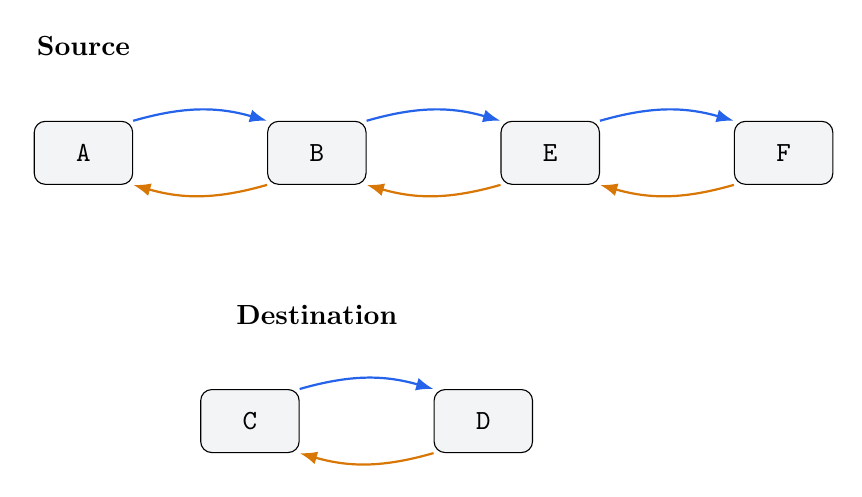
\begin{tikzpicture}[
    node distance=1.7cm,
    listnode/.style={
        draw,
        rounded corners,
        minimum width=1.25cm,
        minimum height=0.8cm,
        fill=listnodefill,
        font=\ttfamily
    },
    nextlink/.style={
        -{Latex[length=2.2mm]},
        thick,
        listnext
    },
    previouslink/.style={
        -{Latex[length=2.2mm]},
        thick,
        listprevious
    }
]
    \node[font=\bfseries] (sourceLabel) {Source};
    \node[listnode, below=0.7cm of sourceLabel] (a) {A};
    \node[listnode, right=of a] (b) {B};
    \node[listnode, right=of b] (e) {E};
    \node[listnode, right=of e] (f) {F};

    \draw[nextlink] (a.north east) to[bend left=16] (b.north west);
    \draw[nextlink] (b.north east) to[bend left=16] (e.north west);
    \draw[nextlink] (e.north east) to[bend left=16] (f.north west);

    \draw[previouslink] (b.south west) to[bend left=16] (a.south east);
    \draw[previouslink] (e.south west) to[bend left=16] (b.south east);
    \draw[previouslink] (f.south west) to[bend left=16] (e.south east);

    \node[font=\bfseries, below=1.4cm of b] (destinationLabel) {Destination};
    \node[listnode, below=0.7cm of destinationLabel, xshift=-0.85cm] (c) {C};
    \node[listnode, right=of c] (d) {D};

    \draw[nextlink] (c.north east) to[bend left=16] (d.north west);
    \draw[previouslink] (d.south west) to[bend left=16] (c.south east);
\end{tikzpicture}
\end{center}

The internal relationship between \mintinline{text}{C} and \mintinline{text}{D} does not need to be rebuilt.

The important structural changes happen at the boundaries of the extracted range:

\begin{itemize}
    \item \mintinline{text}{B} must connect forwards to \mintinline{text}{E};
    \item \mintinline{text}{E} must connect backwards to \mintinline{text}{B};
    \item \mintinline{text}{C} becomes the first node of the destination;
    \item \mintinline{text}{D} becomes the last node of the destination.
\end{itemize}

\begin{reflectionbox}
Why is this operation able to transfer the range without creating new nodes?

Which two relationships reconnect the source List after the range is detached?
\end{reflectionbox}


\subsection{Implement the Core Extraction Case}

Begin with the interior case only:

\begin{terminal}
make
./bin/test02_new_features "[extract][core]"
\end{terminal}

Read the test before writing code.

Identify:

\begin{itemize}
    \item the source values before extraction;
    \item the inclusive positions being extracted;
    \item the expected source List afterwards;
    \item the expected destination List;
    \item the forward and backward traversal checks.
\end{itemize}

Then implement the smallest amount of code required to make this test pass.

\begin{importantnote}
Do not begin with the boundary cases.

The interior case lets you concentrate on reconnecting two neighbouring nodes without also changing the first or last boundary pointers.
\end{importantnote}

After each change, rerun:

\begin{terminal}
make
./bin/test02_new_features "[extract][core]"
make test01
\end{terminal}

Do not continue until both commands pass.


\subsection{Extend to the Boundary Cases}

Once the interior extraction is green, run:

\begin{terminal}
./bin/test02_new_features "[extract][boundary]"
\end{terminal}

These tests introduce three additional situations:

\begin{itemize}
    \item the extracted range begins at the first node;
    \item the extracted range ends at the last node;
    \item the extracted range contains the entire source List.
\end{itemize}

For each case, ask:

\begin{itemize}
    \item Does the source still have a first node?
    \item Does the source still have a last node?
    \item Which boundary pointers must now change?
    \item What should the source size become?
\end{itemize}

\begin{commonerror}
\textbf{Handling only the interior case}

An implementation may correctly reconnect two interior neighbours but fail when one of those neighbours does not exist.

If the extracted range starts at position \mintinline{cpp}{0}, there is no node before it.

If it ends at the final position, there is no node after it.

If the entire List is extracted, both source boundary pointers must become \mintinline{cpp}{nullptr}.
\end{commonerror}

Continue making small changes until:

\begin{terminal}
make
./bin/test02_new_features "[extract][core]"
./bin/test02_new_features "[extract][boundary]"
make test01
\end{terminal}

all pass.


\subsection{Verify Defensive Behaviour}

Finally, run:

\begin{terminal}
make
./bin/test02_new_features "[extract][defensive]"
\end{terminal}

These tests should already pass if your validation remains at the beginning of the function.

Confirm that invalid requests:

\begin{itemize}
    \item return \mintinline{cpp}{false};
    \item leave the source unchanged;
    \item leave the destination unchanged.
\end{itemize}

Then run the complete extraction group:

\begin{terminal}
make
./bin/test02_new_features "[extract]"
\end{terminal}

and the regression suite:

\begin{terminal}
make test01
\end{terminal}

\begin{reflectionbox}
Why should all validation happen before the first link is changed?

How do the backward traversal assertions detect damage that forward traversal alone might hide?
\end{reflectionbox}
% =============================================================================
% Part D
% =============================================================================

\section{Part D: The Grand European Express}

\begin{learningoutcomes}
By the end of this part, you should be able to:

\begin{itemize}
    \item use a generic List to store structured application data;
    \item locate information within a List by traversing its contents;
    \item combine previously implemented List operations to solve a larger engineering problem;
    \item separate application logic from data structure implementation;
    \item reuse an existing abstraction without modifying its implementation.
\end{itemize}
\end{learningoutcomes}

\begin{infobox}[Estimated Effort]
This section should take about 40 minutes to complete.
\end{infobox}


\subsection{From Component to Application}

Throughout this practical you have progressively developed a reusable software component.

In Part A, you observed an existing implementation.

In Part B, you examined how that implementation maintains its internal structure.

In Part C, you extended the component with two new operations.

Part D completes the engineering journey.

Rather than modifying the List implementation again, you will now use it to solve a realistic application problem.

The repository contains a simple railway route planner modelling the \textbf{Grand European Express}, a fictional service connecting more than sixty stations from Portugal to Egypt.

Each station records:

\begin{itemize}
    \item its name;
    \item its country;
    \item its currency;
    \item whether the station is currently affected by scheduled maintenance.
\end{itemize}

Your task is to temporarily suspend part of the route for maintenance before restoring the complete service.


\begin{importantnote}
The implementation of \mintinline{text}{List<T>} should now be complete.

You should not need to modify \mintinline{text}{include/List.h} again.

This part is about reusing the abstraction you have developed, not extending it further.
\end{importantnote}


% -----------------------------------------------------------------------------


\subsection{Explore the Route Planner}

Run:

\begin{terminal}
make run-example03
\end{terminal}

The program loads the complete route from:

\begin{terminal}
data/stations.txt
\end{terminal}

and displays every station together with its associated information.

Spend a few moments exploring the output before examining the implementation.

Notice that the route is now represented as:

\begin{cppcode}
List<Station>
\end{cppcode}

rather than

\begin{cppcode}
List<std::string>
\end{cppcode}

used earlier in the practical.

This demonstrates one of the principal advantages of generic programming.

The List implementation has not changed.

Only the type of object being stored has changed.


% -----------------------------------------------------------------------------


\subsection{The Engineering Problem}

A section of the Grand European Express is about to undergo scheduled maintenance.

Stations marked with the maintenance flag should be temporarily removed from the operational route and placed into a second List representing the suspended section.

Once maintenance has been completed, that section should be restored to exactly the same position in the original route.

\begin{engineeringquestion}
How can an entire section of railway be suspended and later restored without deleting or recreating any station records?
\end{engineeringquestion}

Figure~\ref{fig:route-overview} shows the conceptual route used throughout this exercise.

\begin{figure}[htbp]
    \centering

    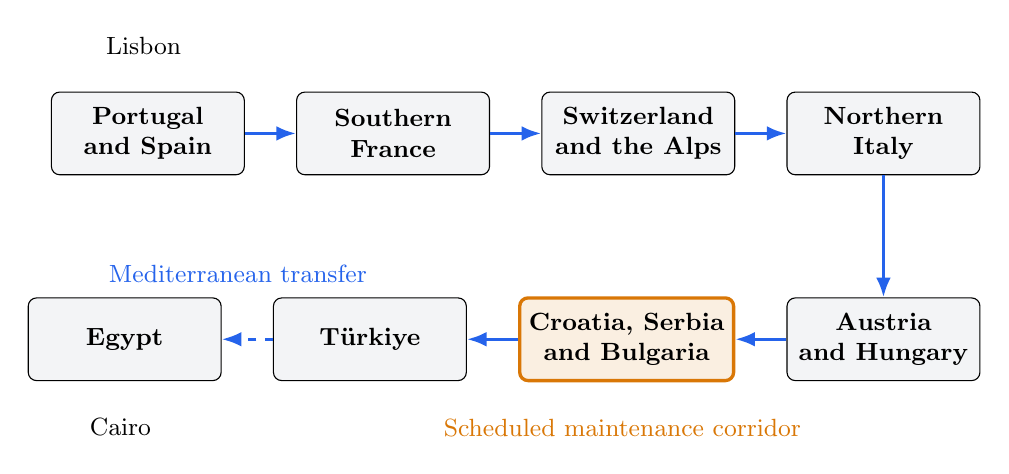
\begin{tikzpicture}[
        region/.style={
            draw,
            rounded corners=3pt,
            minimum width=2.45cm,
            minimum height=1.05cm,
            align=center,
            fill=listnodefill,
            font=\small\bfseries
        },
        maintenance/.style={
            region,
            draw=listprevious,
            very thick,
            fill=listprevious!12
        },
        routearrow/.style={
            -{Latex[length=2.5mm]},
            very thick,
            listnext
        },
        ferryarrow/.style={
            -{Latex[length=2.5mm]},
            very thick,
            dashed,
            listnext
        },
        annotation/.style={
            font=\small,
            align=center
        }
    ]

        % ---------------------------------------------------------------------
        % First row: Western and Central Europe
        % ---------------------------------------------------------------------

        \node[region] (iberia) {Portugal\\and Spain};

        \node[
            region,
            right=0.65cm of iberia
        ] (france) {Southern\\France};

        \node[
            region,
            right=0.65cm of france
        ] (alps) {Switzerland\\and the Alps};

        \node[
            region,
            right=0.65cm of alps
        ] (italy) {Northern\\Italy};

        \draw[routearrow]
            (iberia.east) -- (france.west);

        \draw[routearrow]
            (france.east) -- (alps.west);

        \draw[routearrow]
            (alps.east) -- (italy.west);


        % ---------------------------------------------------------------------
        % Second row: Central Europe to Egypt
        % ---------------------------------------------------------------------

        \node[
            region,
            below=1.55cm of italy
        ] (central) {Austria\\and Hungary};

        \node[
            maintenance,
            left=0.65cm of central
        ] (balkans) {Croatia, Serbia\\and Bulgaria};

        \node[
            region,
            left=0.65cm of balkans
        ] (turkiye) {Türkiye};

        \node[
            region,
            left=0.65cm of turkiye
        ] (egypt) {Egypt};

        % Turn from the first row into the second row.
        \draw[routearrow]
            (italy.south)
            -- ++(0,-0.45cm)
            -| (central.north);

        % Continue eastwards conceptually, while the second row reads
        % from right to left to keep the figure compact.
        \draw[routearrow]
            (central.west) -- (balkans.east);

        \draw[routearrow]
            (balkans.west) -- (turkiye.east);

        % Dashed connection represents the Mediterranean transfer.
        \draw[ferryarrow]
            (turkiye.west) -- (egypt.east);


        % ---------------------------------------------------------------------
        % Labels and annotations
        % ---------------------------------------------------------------------

        \node[
            annotation,
            above=0.35cm of iberia
        ] {
            Lisbon
        };

        \node[
            annotation,
            below=0.35cm of egypt
        ] {
            Cairo
        };

        \node[
            annotation,
            text=listprevious,
            below=0.35cm of balkans
        ] {
            Scheduled maintenance corridor
        };

        \node[
            annotation,
            text=listnext,
            above=0.6cm of $(turkiye.west)!0.6!(egypt.east)$
        ] {
            Mediterranean transfer
        };

    \end{tikzpicture}

    \caption{
        The Grand European Express route. The highlighted Balkan corridor
        contains the stations affected by scheduled maintenance.
    }
    \label{fig:route-overview}
\end{figure}

The diagram shows only the broad regional journey. The complete sequence of
stations and their operating status is stored in
\mintinline{text}{data/stations.txt}.


% -----------------------------------------------------------------------------


\subsection{Understand the Starting Point}

Open:

\begin{terminal}
examples/example03_route_planner.cpp
\end{terminal}

Most of the application has already been implemented.

The program:

\begin{itemize}
    \item loads every station from the input file;
    \item constructs the complete railway route;
    \item displays the current route.
\end{itemize}

Your remaining work consists of three small engineering tasks.

\begin{enumerate}
    \item Locate the maintenance section.
    \item Extract the affected stations.
    \item Restore the original route.
\end{enumerate}


% -----------------------------------------------------------------------------


\subsection{Task 1: Locate the Maintenance Section}

Open:

\begin{terminal}
tests/test03_route_planner.cpp
\end{terminal}

As in Part C, the required behaviour has already been described for you.

Begin by running:

\begin{terminal}
make
make test03
\end{terminal}

Read the failing test before writing any code.

Implement:

\begin{cppcode}
find_maintenance_range(...)
\end{cppcode}

This helper should identify the first and last stations whose maintenance flag is set.

No List modifications occur during this stage.

You are simply traversing the route and recording the affected range.

\begin{tipbox}
Solve this task first.

Once the maintenance range has been identified correctly, the remaining application becomes considerably simpler.
\end{tipbox}


% -----------------------------------------------------------------------------


\subsection{Task 2: Suspend the Route}

Once the maintenance range has been identified, reuse the operation you implemented in Part C:

\begin{cppcode}
extract(...)
\end{cppcode}

The extracted stations should become a second List representing the suspended section of railway.

Display both Lists.

Verify that:

\begin{itemize}
    \item the operational route no longer contains the maintenance section;
    \item the suspended route contains exactly the extracted stations;
    \item both Lists remain valid.
\end{itemize}


% -----------------------------------------------------------------------------


\subsection{Task 3: Restore the Route}

Finally, reuse the second operation developed in Part C:

\begin{cppcode}
insert(...)
\end{cppcode}

Restore the suspended section to its original position.

Display the complete route once more.

The restored route should match the original output produced when the application first started.

\begin{importantnote}
No new List algorithms are required.

The entire restoration process should reuse the operations you have already implemented and tested.
\end{importantnote}


% -----------------------------------------------------------------------------


\subsection{Verify the Complete Workflow}

Once all three tasks have been completed successfully, run:

\begin{terminal}
make
make test03
\end{terminal}

Finally, confirm that Parts C and D have not accidentally broken any existing functionality:

\begin{terminal}
make test01
make test02
make test03
\end{terminal}

All three test suites should now pass.


% -----------------------------------------------------------------------------


\begin{reflectionbox}

Throughout this practical you have:

\begin{itemize}
    \item inherited an existing software component;
    \item understood its internal design;
    \item extended its functionality;
    \item reused it to solve a realistic engineering problem.
\end{itemize}

Which of these stages did you find the most challenging?

Why is the ability to reuse an existing abstraction generally more valuable than repeatedly writing new implementations from scratch?

\end{reflectionbox}


\subsection{Engineering Takeaway}

\begin{importantnote}
Well-designed software components become more valuable over time.

Once thoroughly tested, a reusable abstraction allows increasingly sophisticated applications to be built without revisiting its internal implementation.

This separation between component development and application development lies at the heart of modern software engineering.
\end{importantnote}

% =============================================================================
% Fast Finisher Challenges
% =============================================================================

\section{Fast Finisher Challenges}

If you have completed all four parts of the practical and your test suites are passing, consider extending the route planner further.

These challenges are entirely optional but provide an opportunity to practise applying the List abstraction to new problems.


\subsection*{Challenge 1: Detect Currency Changes}

Traverse the complete railway route and identify every point where the operating currency changes.

For example:

\begin{terminal}
EUR -> TRY
Between Svilengrad and Edirne

TRY -> EGP
Between Istanbul and Alexandria
\end{terminal}

Think carefully about:

\begin{itemize}
    \item how to compare neighbouring stations;
    \item how to avoid reporting duplicate transitions;
    \item how to produce meaningful output for the user.
\end{itemize}

No modifications to \mintinline{cpp}{List<T>} should be required.


\subsection*{Challenge 2: Build a Currency Index}

Create a new:

\begin{cppcode}
List<std::string> currencies;
\end{cppcode}

containing every distinct currency encountered along the route.

Each currency should appear only once, regardless of how many stations use it.

Consider:

\begin{itemize}
    \item how to determine whether a currency is already present;
    \item where the search should begin;
    \item how generic programming allows the same List implementation to store completely different data types.
\end{itemize}


\begin{tipbox}
Neither challenge requires any changes to the List implementation.

The objective is to continue developing your application by reusing the abstraction you have already built.
\end{tipbox}

% =============================================================================
% Reflection
% =============================================================================

\frontsection{Looking Back}

Over the course of this practical you have followed the complete lifecycle of a reusable software component.

You began by observing an existing implementation before examining how it worked internally.

You then extended that implementation with new functionality while protecting its existing behaviour through regression tests.

Finally, you reused the completed abstraction to solve a realistic engineering problem without modifying its implementation further.

\begin{reflectionbox}

Consider the following questions.

\begin{itemize}
    \item Which part of the practical challenged your understanding the most?
    \item How did the public tests help guide your implementation?
    \item Why is preserving existing behaviour just as important as adding new functionality?
    \item What advantages did the generic List provide when moving from simple strings to structured Station records?
\end{itemize}

\end{reflectionbox}

% =============================================================================
% Engineering Takeaway
% =============================================================================

\frontsection{Engineering Takeaway}

\begin{importantnote}

Throughout this module you have been developing reusable software components.

This practical demonstrated that the true value of an abstraction is not measured by how difficult it was to implement, but by how easily it can be reused.

A well-designed component can be:

\begin{itemize}
    \item understood without exposing unnecessary implementation details;
    \item extended while preserving existing behaviour;
    \item reused in applications that its original designer may never have anticipated.
\end{itemize}

These principles underpin modern software engineering, where reliable systems are built by combining well-tested, reusable components rather than repeatedly reinventing them.

\end{importantnote}


You have completed Practical 6.

Take a moment to appreciate how far you have come since the beginning of the module. You are no longer simply writing individual functions—you are engineering reusable software.  Congratulations!

\end{document}